\chapter{Distribuited Brute Force}

Per poter migliorare l'efficenza dei attacchi di Brute Force, oltre all'utilizzo di CUDA, sono stati creati dei strumenti che attraverso la rete, permettono di unire la potenza computazionale di diverse macchine, in modo da distribuire il carico di lavoro dei processi più complessi.

Nella rete possiamo trovare diversi strumenti che ci permettono di eseguire questo tipo di operazione, come per esempio Hashtopolis, Hashstack, Disthc , ecc ecc.

\section{Hashtopolis}

Hashtopolis \cite{hashtopolis} è un applicazione multi piattaforma per il cracking distribuito che nasce nel 2018. L’applicazione utilizza per la parte di cracking Hashcat il quale viene installato on-demand per mezzo degli agent. 

\begin{figure}[ht]
    \centering
    
\includegraphics[width=50mm]{Immagini/8/hashtopoli_logo.png}
    \caption{hashcat Logo}
\end{figure}

La potenzialità maggiore del progetto è la portabilità, infatti gli autori hanno scelto come linguaggi di sviluppo python e php. Ha una gestione utenti e gruppi granulare che arriva a definire una serie di caratteristiche come ad esempio la disponibilità del numero di nodi di rete per il cracking a seconda del profilo.

Hashtopolis è composto da 2 parti:

\begin{itemize}
    \item \textbf{Agent} Disponibili in Python. Quindi supportati da Windows, OSx e Linux.
    \item \textbf{Server} Opera con due GUI la parte di Admin e quella relativa agli Agent Connection Point. Il database di backend è in Mysql.
\end{itemize}

La comunicazione tra agent e server avviene attraverso il protocollo HTTP(S) il che aggiunge un punto in più sulla portabilità. Non necessita quindi di aprire ulteriori porte di rete.

L’interfaccia di Admin è l’unico punto di accesso per tutti gli agent. Il collegamento di un nuovo agent è molto semplice e richiede la generazione di una one-time password. 

\begin{figure}[ht]
    \centering
    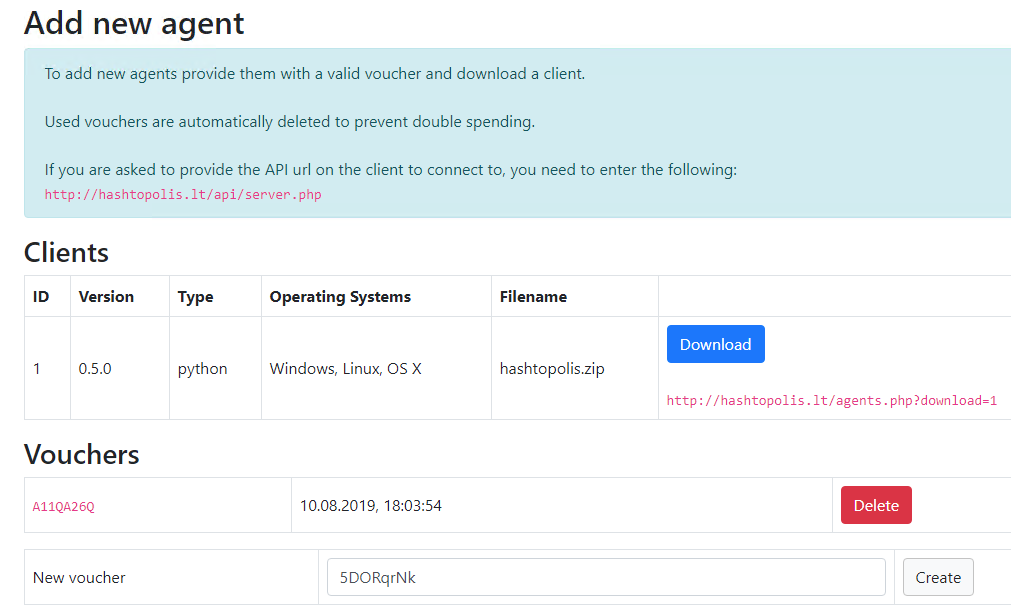
\includegraphics[width=\linewidth]{Immagini/8/hashtopolis_new_agent.png}
    \caption{Hashtopolis aggiunta di nuovi aggenti}
\end{figure}

Successivamente dobbiamo caricare nella piattaforma il file su cui eseguire l'attacco, andando a specificare il tipo di criptazione applicata su quei dati ed eventuali parametri passati.

\begin{figure}[ht]
    \centering
    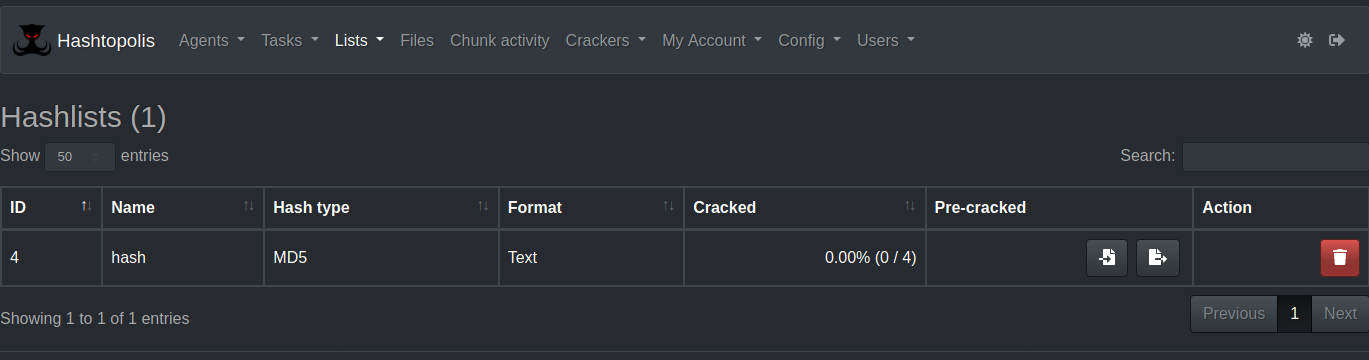
\includegraphics[width=\linewidth]{Immagini/8/hashtopolis_2.png}
    \caption{Hashtopolis aggiunta lista hash da attaccare}
\end{figure}

Hashtopolis ci peremtte di eseguire diversi tipi di attacco, per esempio possiamo eseguire attacchi Ruled based o Dictionary Attack, ma per eseguire questi tipi di attacchi, dobbiamo passare dei file di "configurazione", in questo caso noi per eseguire un Dictionary Attack, gli passiamo il dizionario rockyou, uno dei dizionari più utilizzati per eseguire questo tipo di operazione.

\begin{figure}[ht]
    \centering
    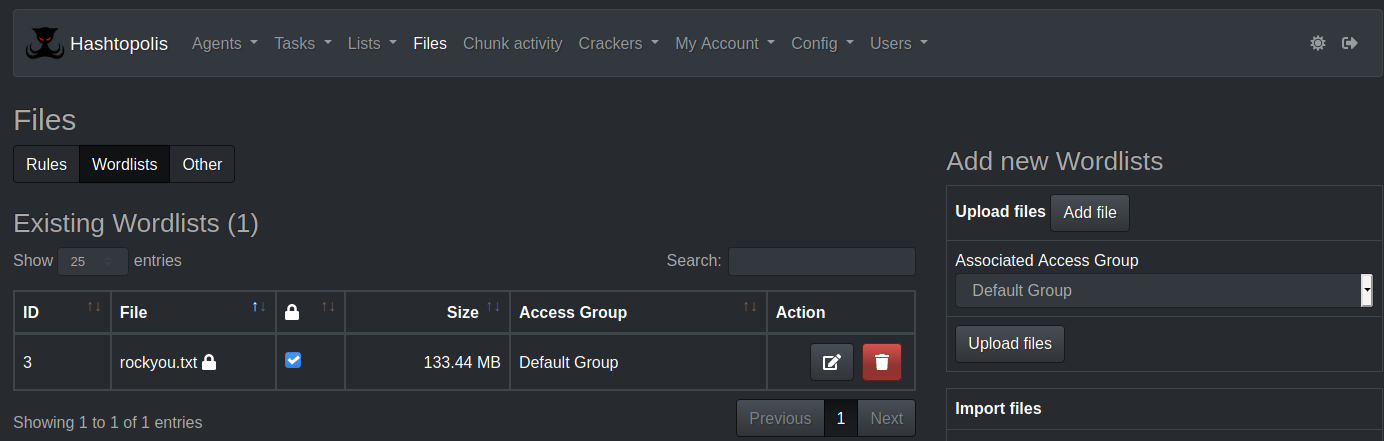
\includegraphics[width=\linewidth]{Immagini/8/hashtopolis_3.png}
    \caption{Hashtopolis aggiunta dizionario}
\end{figure}

Una volta configurati i file di cui si ha bisogno per eseguire l'attacco, si passa alla creazione della task, qui andremo ad associare :
\begin{itemize}
    \item un nome
    \item una lista di hash su cui eseguire il crack
    \item il dizionario/file delle regole
    \item priorità dell'attacco
    \item utilizzo di CPU, GPU o entrambe
    \item Gruppo che può eseguire l'attacco 
    \item ecc ecc 
\end{itemize}

\begin{figure}[ht]
    \centering
    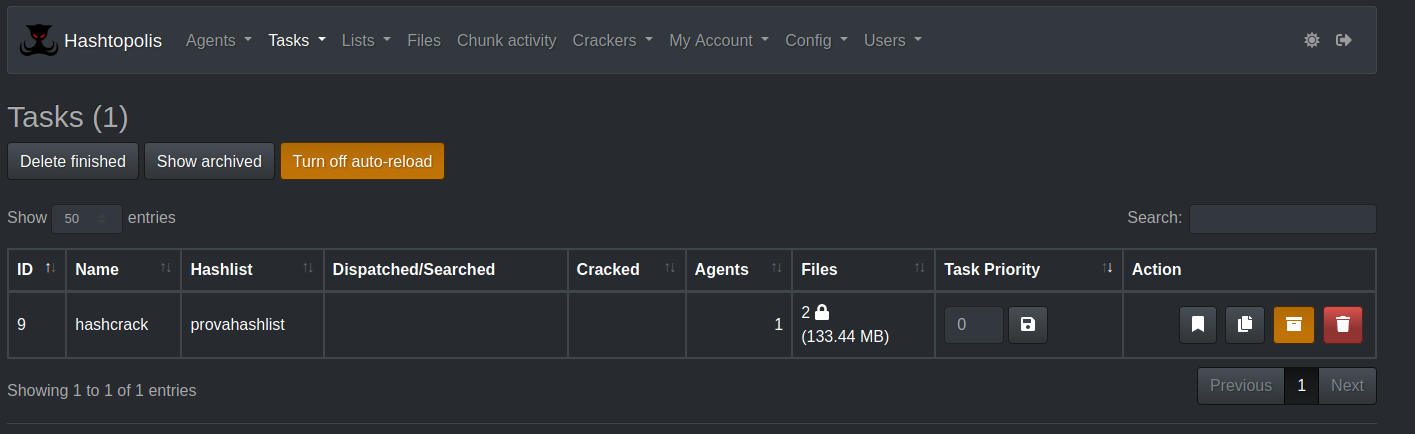
\includegraphics[width=\linewidth]{Immagini/8/hashtopolis_1.png}
    \caption{Hashtopolis creazione task}
\end{figure}

Dopo aver creato la task, ora possiamo andare ad associargli dei utenti, in modo da poter utilizzare la loro potenza di calcolo per eseguire l'attacco.

\begin{figure}[ht]
    \centering
    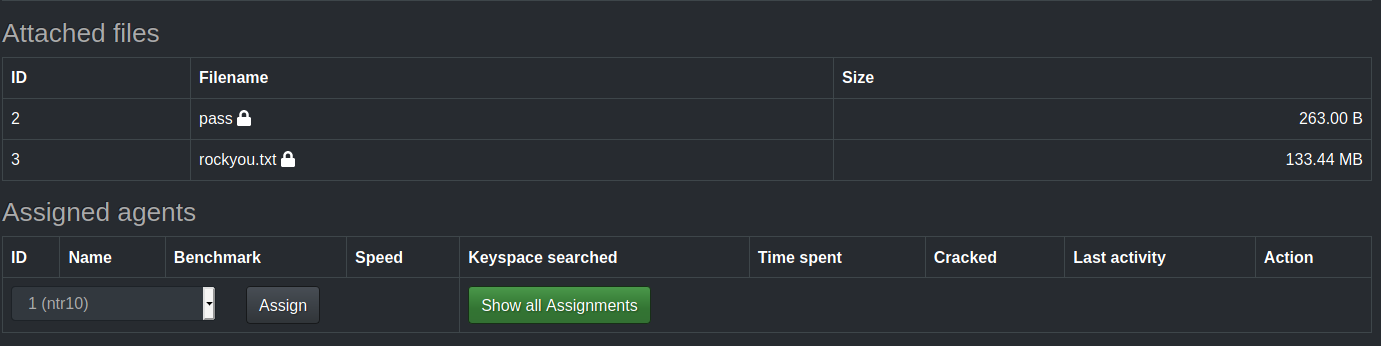
\includegraphics[width=\linewidth]{Immagini/8/hashtopolis_4.png}
    \caption{Hashtopolis aggiunta user a task}
\end{figure}

Una volta che uno user è stato associato ad una task, questo potrà eseguire lo script python, che lo colleghera al server e questo in automatico gli passerà i dati di cui ha bisogno per eseguire l'attacco e lui inizierà ad eseguire le varie operazioni.

\begin{figure}[ht]
    \centering
    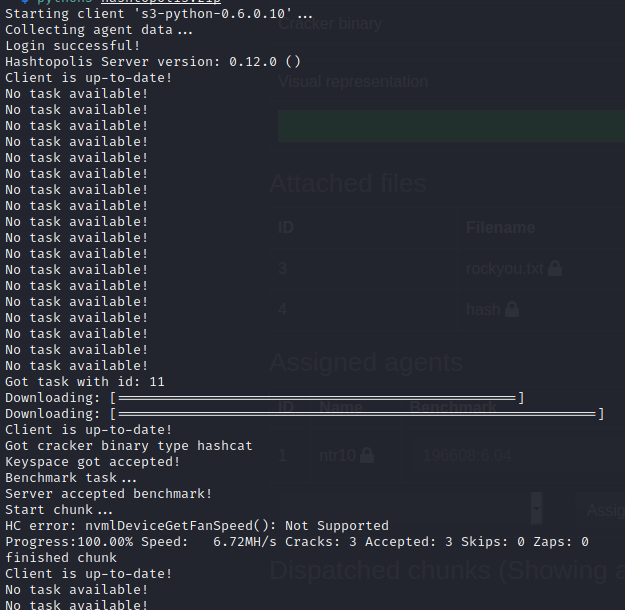
\includegraphics[width=\linewidth]{Immagini/8/hashtopolis_8.png}
    \caption{Hashtopolis client script}
\end{figure}

Dopo che l'utente avrà completato l'operazione, possiamo vedere nel sito di hashtopolis tutti i dati inerenti al crack, in modo da visualizzare quanti hash rimangono e quali sono stati risolti e quali ancora devono essere controllati.

\begin{figure}[ht]
    \centering
    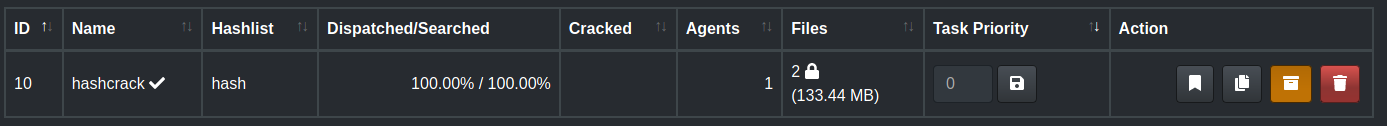
\includegraphics[width=\linewidth]{Immagini/8/hashtopolis_6.png}
    \caption{Hashtopolis task conclusa}
\end{figure}

All'interno di ogni task, possiamo vedere la suddivisione del lavoro tra i vari user che sono stati aggiunti alla task, qui possiamo vedere quanti hash hanno risolto e il tempo di esecuzione.
\newpage
\begin{figure}[ht]
    \centering
    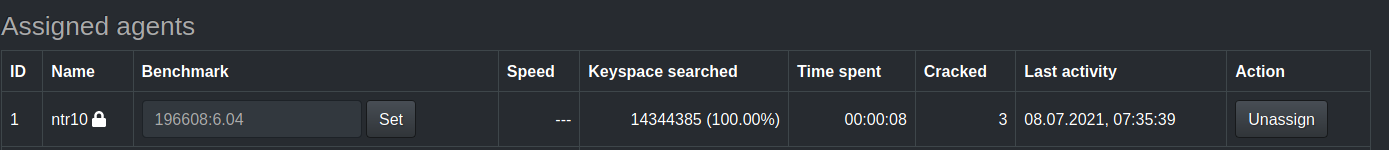
\includegraphics[width=\linewidth]{Immagini/8/hashtopolis_9.png}
    \caption{Hashtopolis suddivisione lavoro task per agent}
\end{figure}

Infine, una volta completata l'operazione, possiamo andare nella sezione hashlist, per visualizzare le password scoperte e quelle che ancora non sono state risolte.

\begin{figure}[ht]
    \centering
    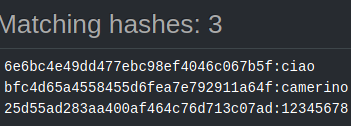
\includegraphics[width=\linewidth]{Immagini/8/hashtopolis_10.png}
    \caption{Hashtopolis password estratte}
\end{figure}

\label{chap:conc}